\documentclass{beamer}
\usepackage[german,english]{babel}
\usepackage[utf8]{inputenc}

\usepackage{graphicx}
\usepackage{etoolbox}
\makeatletter
\patchcmd{\Ginclude@eps}{"#1"}{#1}{}{}
\makeatother
%\usepackage{wrapfig}
%\usepackage{eurosym}
%\usepackage{tabularx}
%\usepackage{multirow}
%\usepackage{listings}
%\usepackage{color}
\usetheme{metropolis}
% Other valid themes
%   Antibes, Bergen, Berkeley, Berlin, Copenhagen
%   Darmstadt, Dresden, Frankfurt, Goettingen, Hannover
%   Ilmenau, JuanLesPins, Luebeck, Madrid, Malmoe
%   Marburg, Montpellier, PaloAlto, Pittsburgh, Rochester
%   Singapore, Szeged, Warsaw, boxes, default

% \usecolortheme{default}
% Other valid color schemes
%    albatross, beaver, beetle, crane, dolphin
%    dove, fly, lily, orchid, rose, seagull
%    seahorse, whale and the one and only wolverine

\title[Project 3]{Project 3}
\subtitle{clustering, dimensionality reduction, and non-monotonous neurons}
\author{Lukas Drexler, Leif Van Holland, Reza Jahangiri,\\Mark Springer, Maximilian Thiessen}
\institute[Universität Bonn]{Rheinische Friedrich-Wilhelms-Universität}
\date{\today}

\begin{document}
	
\begin{frame}%1
	\titlepage
\end{frame}

%no table of contents not enough content for that
%\begin{frame}%2
%\frametitle{Table of Contents}
%\tableofcontents%[pausesections]
%\end{frame}


\section{Task 1.1}

\begin{frame}
\frametitle{Fun with k-means clustering}

\end{frame}

%\begin{frame}
%\frametitle{Results for $d\in \{1,5,10\}$}
%\begin{figure}
%	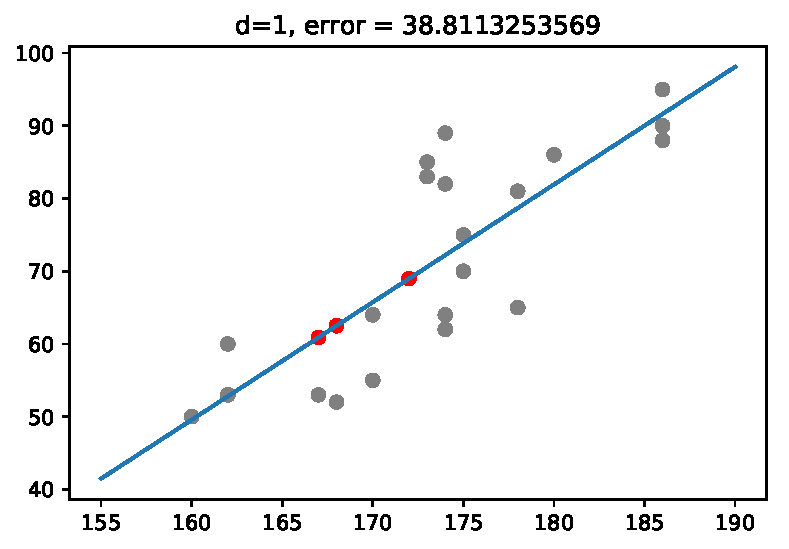
\includegraphics[height=0.5\textheight]{graphics/poly_1_coeffs}
%\end{figure}

\section{Task 3.2}
\begin{frame}
	\frametitle{Spectral clustering}
	Given data, $X = \{x_1,\ldots,x_n\} \subset \mathbb{R}^2$, compute similarity matrix:
	\begin{align*}
		S_{ij} = e^{-\beta ||x_i-x_j||^2}
	\end{align*}
	and the Laplacian $L = D-S$, with diagonal matrix $D$:
	\begin{align*}
	D_{ij} = \begin{cases}
	\sum_j S_{ij} & ,\text{if } i=j\\
	0 &, \text{otherwise}
	\end{cases}\\
	\end{align*}
	Then compute the eigenvalue decomposition of L. Use the eigenvector of the second smallest eigenvalue to partition the data points, according to the sign of the corresponding entry in the eigenvector.
\end{frame}

\begin{frame}
The result using kmeans++:
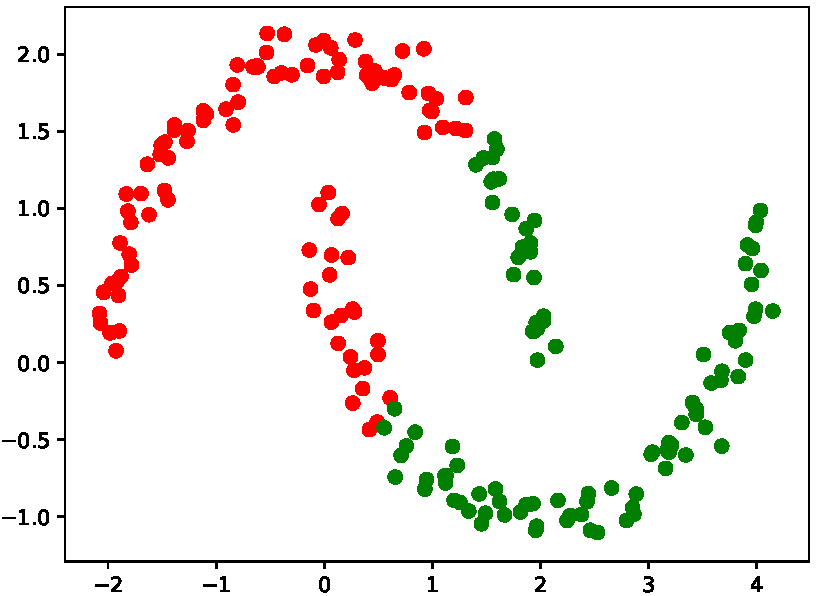
\includegraphics[width=\linewidth]{graphics/task_3_2_kmeans}
\end{frame}
\begin{frame}
	The result using $\beta = 1$ through $4$:
	\begin{overprint}
		\onslide<1>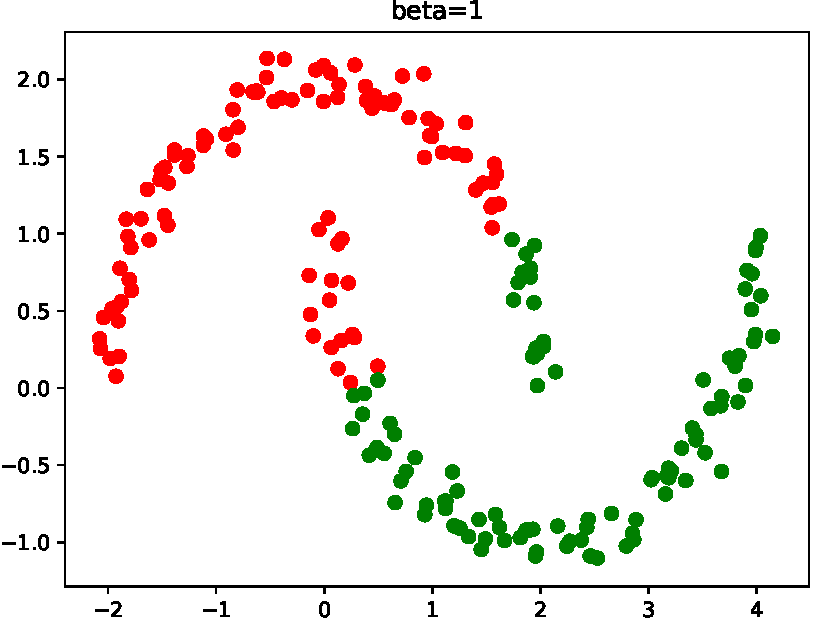
\includegraphics[width=\linewidth]{graphics/task_3_2_spectral1}
		\onslide<2>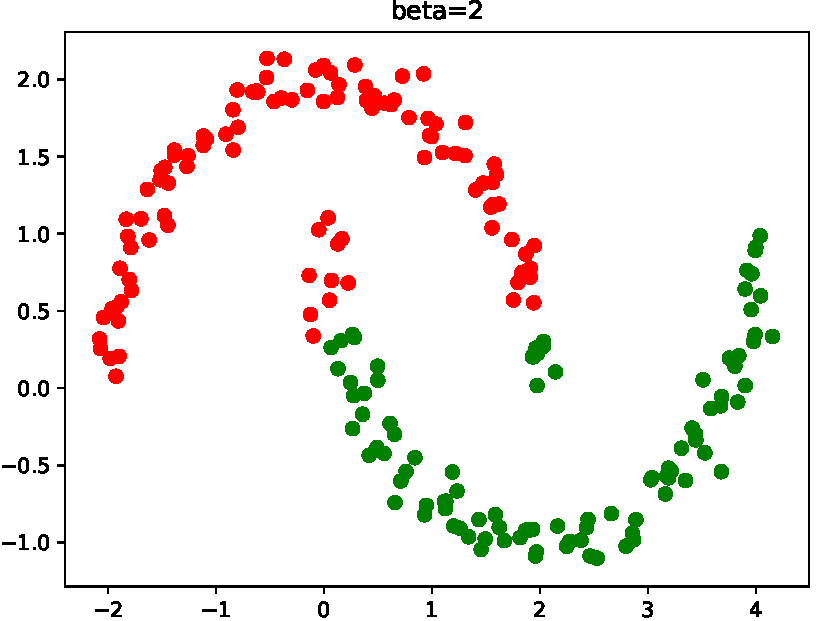
\includegraphics[width=\linewidth]{graphics/task_3_2_spectral2}
		\onslide<3>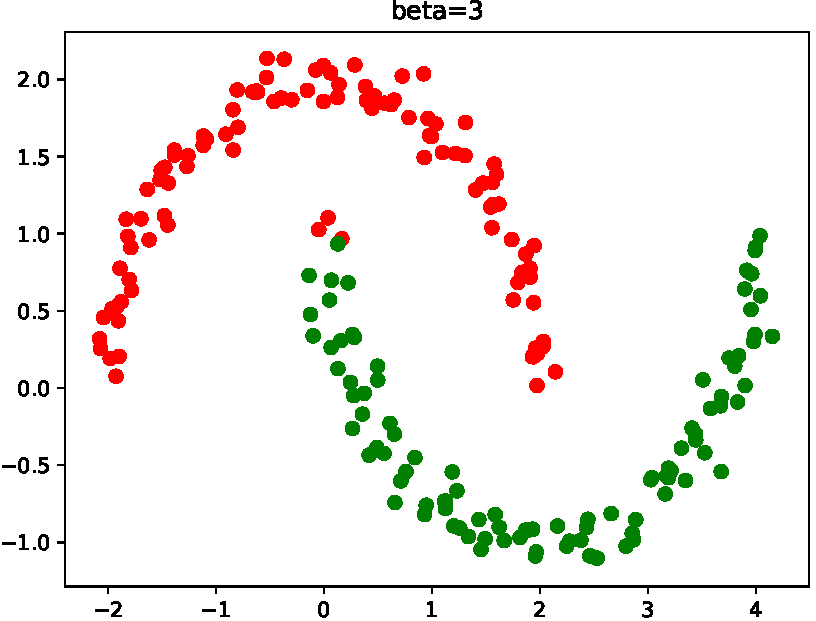
\includegraphics[width=\linewidth]{graphics/task_3_2_spectral3}
		\onslide<4->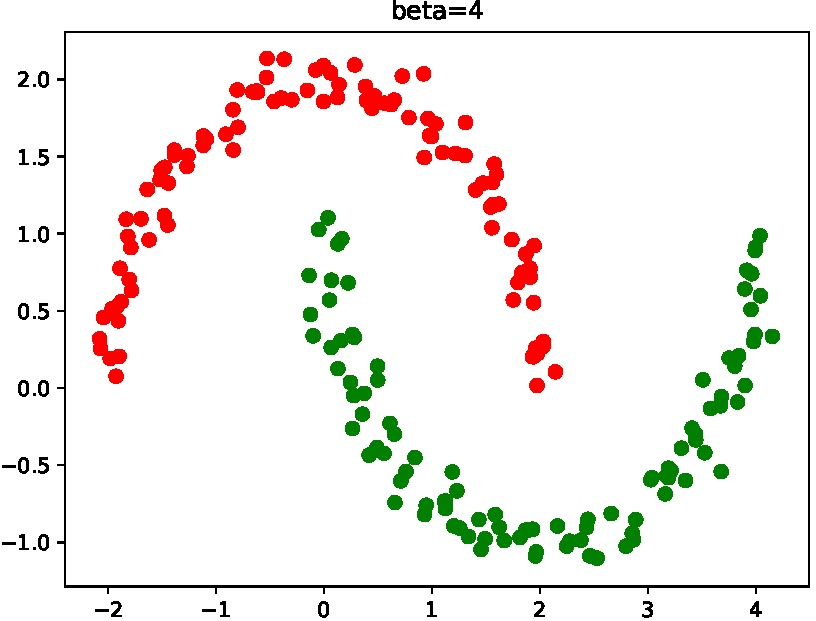
\includegraphics[width=\linewidth]{graphics/task_3_2_spectral4}
	\end{overprint}
\end{frame}

\section{Task 3.3}
\begin{frame}
	\frametitle{Dimensionality reduction}
	This task explores mappings $\mathbb{R}^{500} \to \mathbb{R}^2$, in particular Principal Component Analysis (PCA) and multi-class LDA.
\end{frame}

\begin{frame}
	\frametitle{Dimensionality reduction}
	Idea: Project $n=150$ \emph{zero-mean} data $x_1,...,x_n$ onto eigenvectors $u_1$ and $u_2$ corresponding to largest eigenvalues $\lambda_1 \geq \lambda_2 \geq ... \geq \lambda_n$:
	\begin{itemize}
	\item[PCA:] eigenvectors of sample covariance matrix 
	\[\Sigma = \frac{1}{n+1} \sum_{i=1}^n x_i \cdot x_i^T\]
	\item[LDA:] eigenvectors of
	\[S_W^{-1}S_B = \left(\sum_{j=1}^k \Sigma_j\right)^{-1} \sum_{j=1}^k \mu_j \cdot \mu_j^T\]
	where $\mu_j$ are the mean vectors and $\Sigma_j$ are the covariance matrices for the $k=3$ classes the data points are from
	\end{itemize}
\end{frame}

\begin{frame}
	\frametitle{PCA and LDA in two dimensions}
	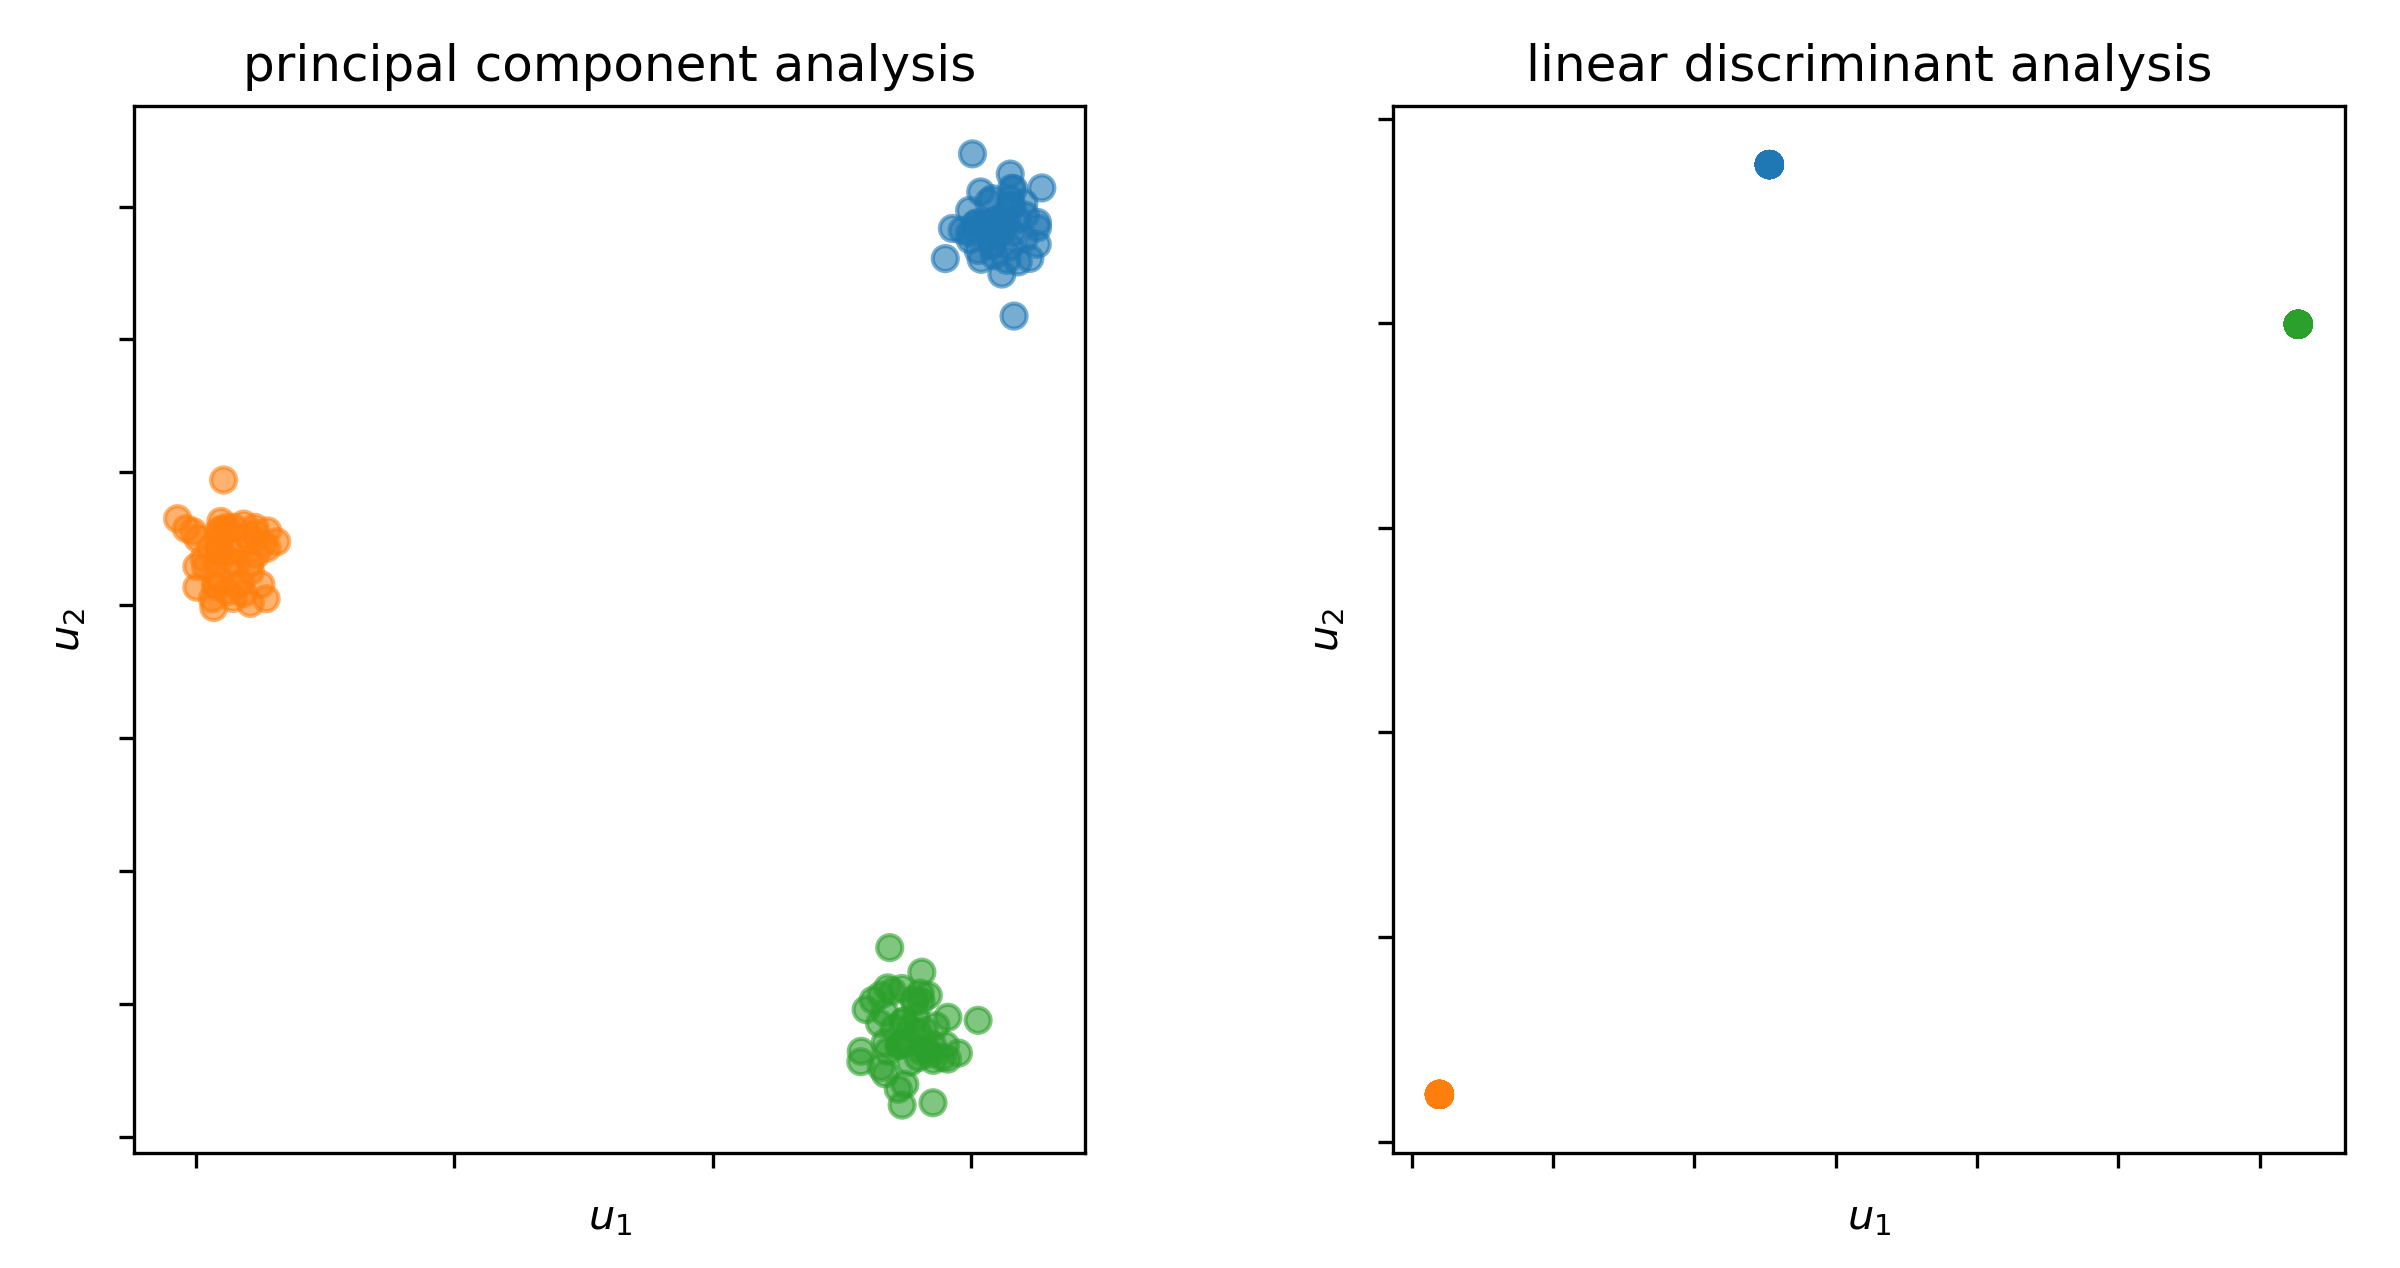
\includegraphics[width=\linewidth]{graphics/pca_lda_2d}
\begin{description}
	\item[Observe:]Data points with same label form clusters\\
	if projected.
\end{description}
\end{frame}

\begin{frame}
	\frametitle{PCA and LDA in three dimensions}
	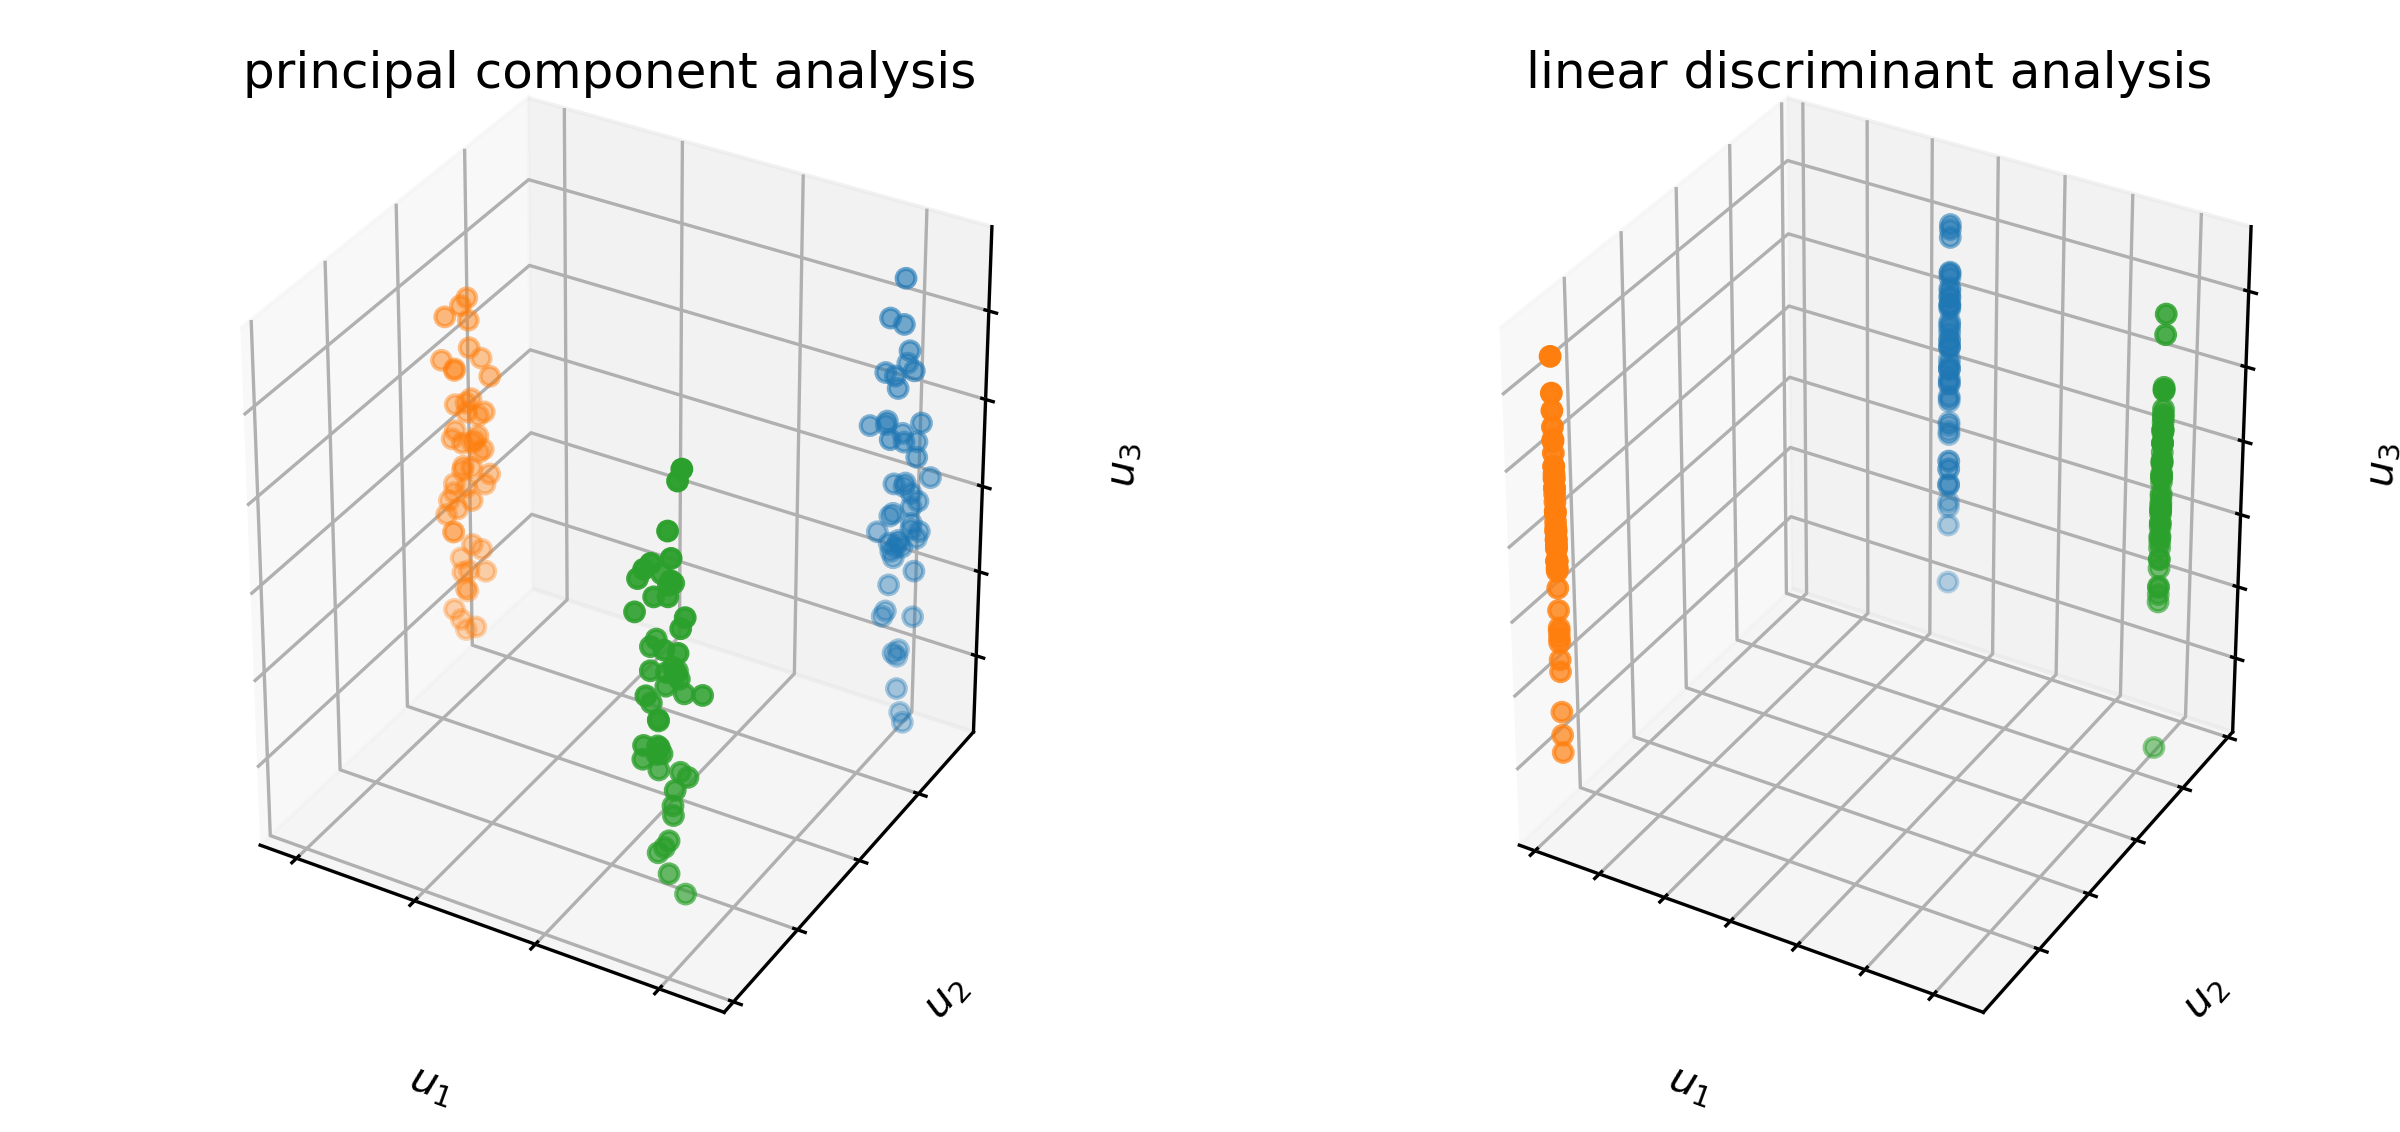
\includegraphics[width=\linewidth]{graphics/pca_lda_3d}
\begin{description}
	\item[Observe:] Data points are (per class) located in a\\
	1D-subspace of $\mathbb{R}^{500}$.
\end{description}
\end{frame}

\begin{frame}
	\frametitle{PCA vs LDA}
	Why do the results differ?\\
\hfill\\
\begin{itemize}
\item[PCA:] Yields axes of maximum variance in complete data set.\\
$\Rightarrow$ Preserves as much \emph{variance} as possible.\hfill\\
\item[LDA:] Uses class labels to maximize distance between class means and minimize class variances.\\
$\Rightarrow$ Preserves as much \emph{discriminatory} information as possible.\\\hfill\\
\end{itemize}
\end{frame}


\section{Task 3.4}
\begin{frame}
	\frametitle{Perceptrons}
	\begin{itemize}
	\item Gradient descent for perceptron learning:
		\begin{itemize}
			\item line search version
			\item use best result of $k$ runs, to prevent local minima
			\item monotonous activation separates only linearly
			\item avoid this limitation with non-monotonous activation 	
		\end{itemize}
	\end{itemize}
\end{frame}
\begin{frame}
	\frametitle{Monotonous Perceptron (tanh)}
	\includegraphics[width=0.5\textwidth]{"graphics/Tanh Activation (init)"}%
	\includegraphics[width=0.5\textwidth]{"graphics/Tanh Activation (best of 1)"}
\end{frame}

\begin{frame}
	\frametitle{Non-monotonous Perceptron (Gaussian)}
	\includegraphics[width=0.5\textwidth]{"graphics/Gaussian Activation (init)"}%
	\includegraphics[width=0.5\textwidth]{"graphics/Gaussian Activation (best of 10)"}
\end{frame}

\begin{frame}
	\frametitle{SVM}
	\begin{itemize}
		\item L2-SVM with polynomial kernel:
		\begin{itemize}
			\item Train with Frank-Wolfe algorithm
			\item $d=2$ (i.e. quadratic kernel) is enough	
		\end{itemize}
	\end{itemize}
\end{frame}
\begin{frame}
	\frametitle{Polynomial Kervel SVM}
	\centering
	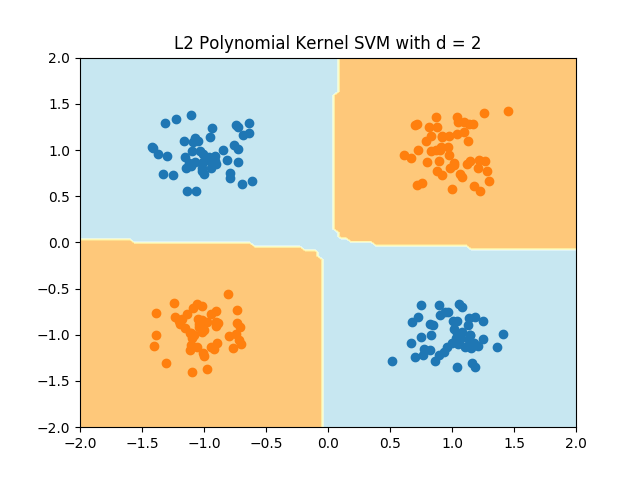
\includegraphics[width=0.9\textwidth]{graphics/svm}%
\end{frame}

\section{Task 3.5}
\begin{frame}
	\frametitle{Exploring numerical instabilities}
\end{frame}


%\bibliography{Bibliography}
%\bibliographystyle{plain}

%\begin{thebibliography}{}
%\bibitem{1} 
%\bibitem{2} 
%\bibitem{3} 
%\end{thebibliography}


\end{document} 
